%%%%%%%%%%%%%%%%%%%%%%%%
%
% $Author: Deepti Hegde $
% $Datum: 2023-06-26  $
% $Pfad: BA23-02-Sales-Predictor/report/Contents/en/TechnicalRequirements.tex $
% $Version: 1.0 $
% $Reviewed by: Deepti, Sadegh and Raunak $
% $Review Date: 2023-07-03 $
%
%%%%%%%%%%%%%%%%%%%%%%%%


\chapter{Technical Requirements}

\section{Hardware Requirements}

\subsection{Material List Required For Sales Prediction project }

Component list required for the Project are:
\begin{enumerate}
	\item Laptop
	\item Monitor
	\item Keyboard
	\item Mouse
	\item HDMI Cable
\end{enumerate}

\subsection{Specifications of Development Environment}

 \textbf{Developement Enviornment:} 
\begin{enumerate}
	\item \textbf{Operating system}: 
	\begin{itemize}
		\item Windows\texttrademark 10 (64 bit) version 22H2 (OS Build 19045.2846)
	\end{itemize}
	
	\item \textbf{Processors}:
	\begin{itemize}
		\item Intel Core i7-4710HQ processor (2.5GHz quad-core with Turbo Boost up to 3.5GHz)
	\end{itemize}
	
		\item \textbf{RAM}:
	\begin{itemize}
		\item 16GB DDR3L 1600 MHz SDRAM
	\end{itemize}

	\item \textbf{Storage}:
\begin{itemize}
	\item 512 GB SSD. A minimum of 100GB of free disk space is recommended.
\end{itemize}

	\item \textbf{GPU}:
\begin{itemize}
	\item NVIDIA GeForce GTX 860M with 4GB GDDR5 VRAM
\end{itemize}

\end{enumerate}


\subsection{Hardware Bill of Material}

\renewcommand{\arraystretch}{1.15}

%\begin{table}
%\begin{longtable}{cp{2.1cm}p{2.5cm}c}
%	\textbf{Quantity} & \textbf{Description} &   \textbf{Link} & \textbf{Price} \\ \hline     
%	\multicolumn{4}{c}{\includegraphics[width=0.2\textwidth]{./Images/Arduino}} \\
%	1      & Arduino Nano 33 BLE Sense 
%	& \href{https://store.arduino.cc/products/arduino-nano-33-ble-sense}{Store.arduino.cc} 
%	&  35{,}1 \texteuro \\ \hline 
%	
%\end{longtable}
%
%\newpage
\begin{longtable}{cp{2.1cm}p{2.5cm}c}
	\multicolumn{4}{c}{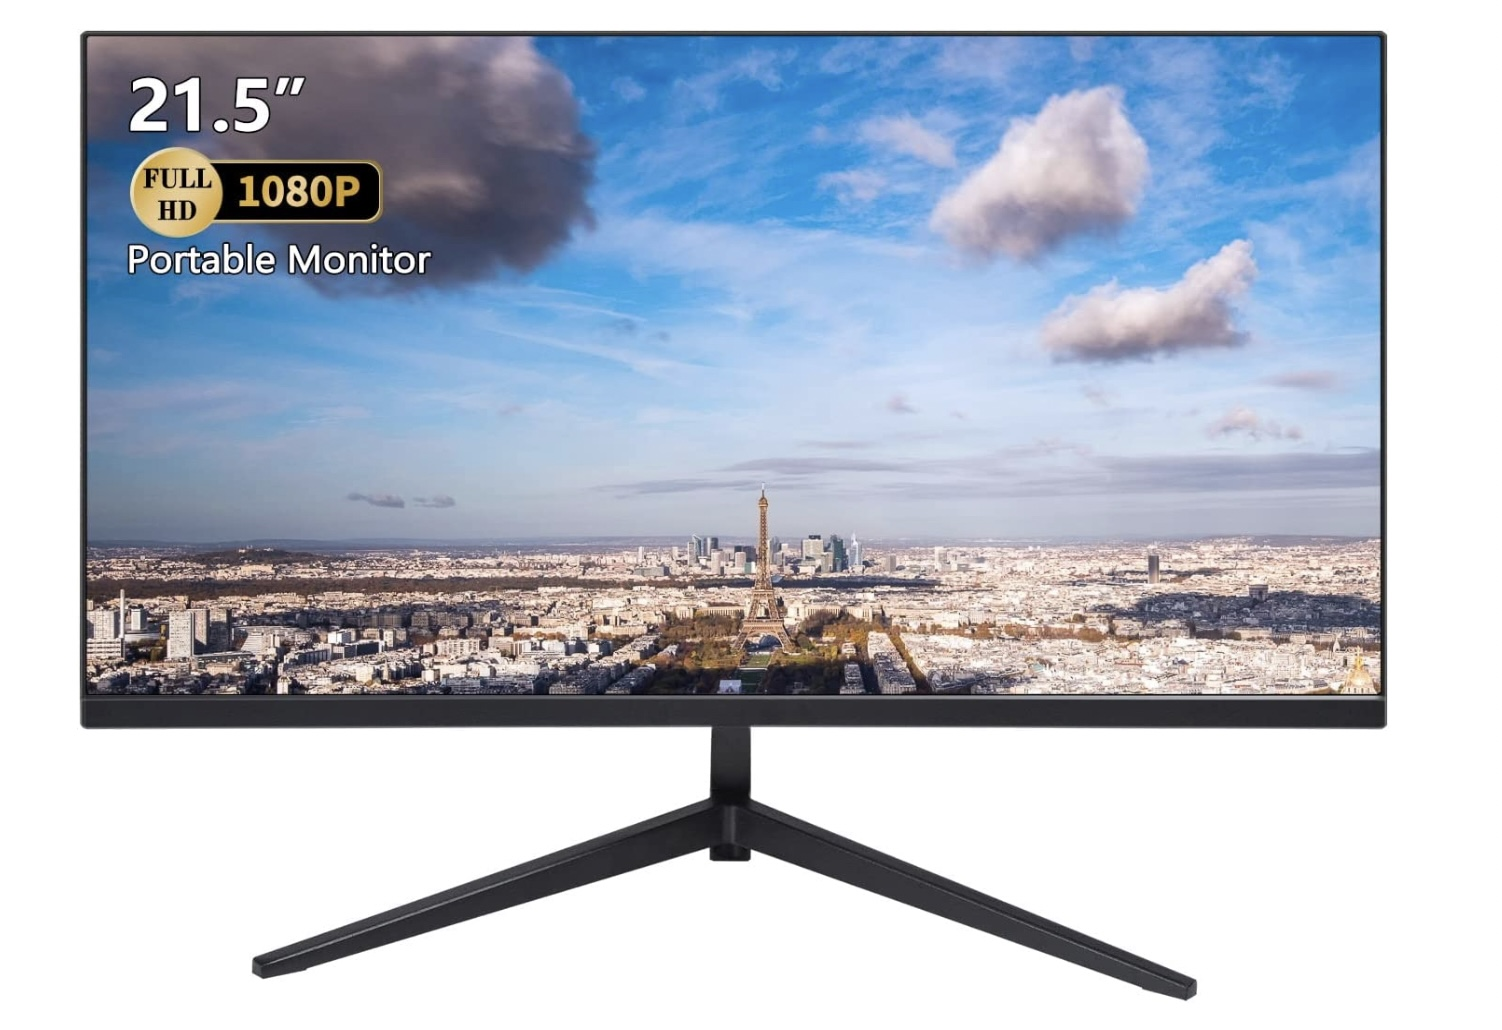
\includegraphics[width=0.2\textwidth]{Images/Monitor}} \\
	1      & Display Monitor 21.5 inch
	& \href{https://www.amazon.de/-/en/Monitor-Frameless-Response-Computer-ZFTVNIE/dp/B09WZY98VB/ref=sr_1_4?crid=9VZ9DMBD4ZMK&keywords=monitor&qid=1675602231&sprefix=monitor%2Caps%2C168&sr=8-4}{Amazon.de} 
	&  94{,}99 \texteuro\\ \hline \\
	
	\multicolumn{4}{c}{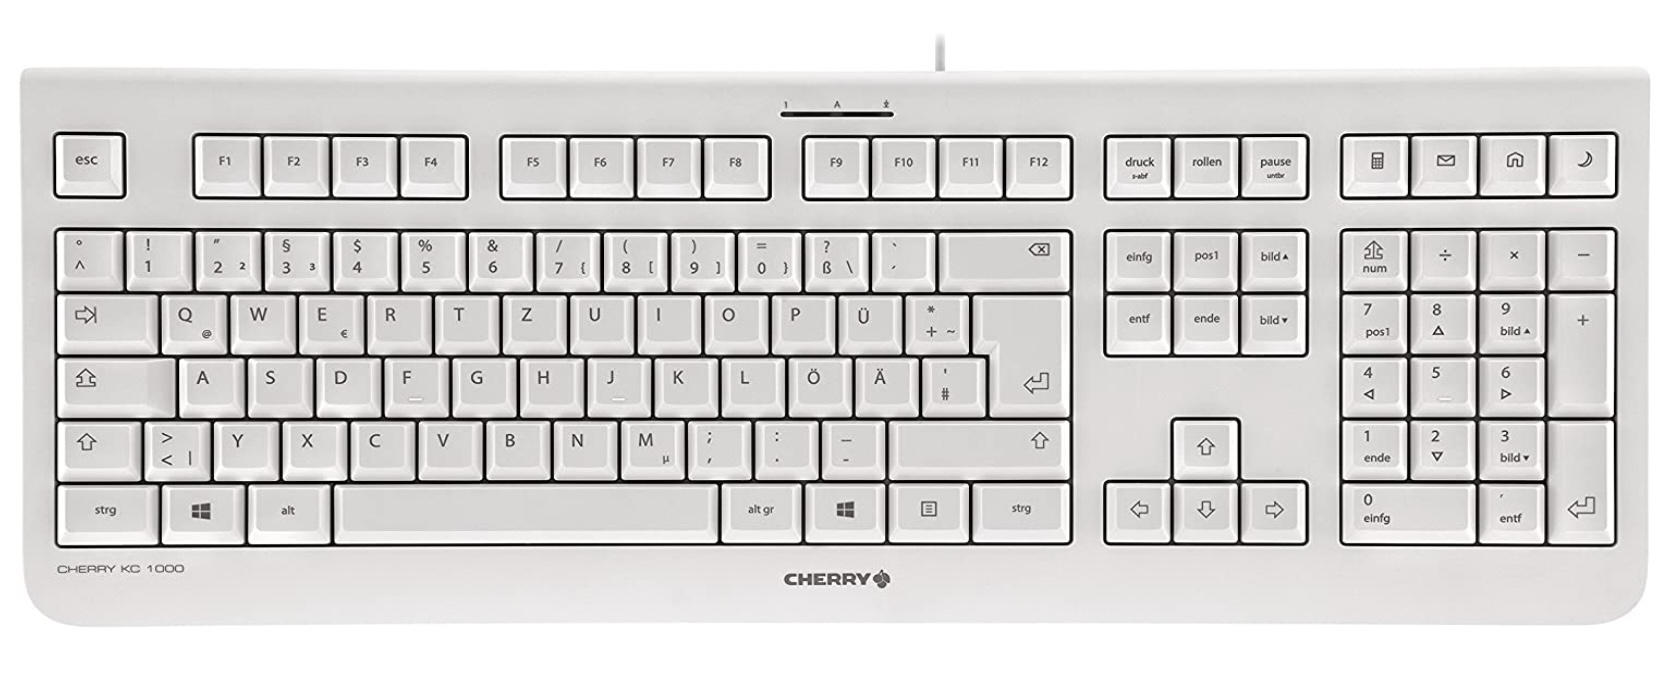
\includegraphics[width=0.2\textwidth]{Images/Keyboard}} \\
	1      &  Wired USB Keyboard  
	& \href{https://www.amazon.de/-/en/Cherry-Keyboard-Approval-Business-white-grey/dp/B00F35N1KS/ref=sr_1_3?crid=2YJGO50SYCWDB&keywords=kabelgebundene+usb+tastatur&qid=1675602753&sprefix=wired+usb+keyboard%2Caps%2C137&sr=8-3}{Amazon.de} 
	&  10{,}99 \texteuro \\ \hline \\
	
	\multicolumn{4}{c}{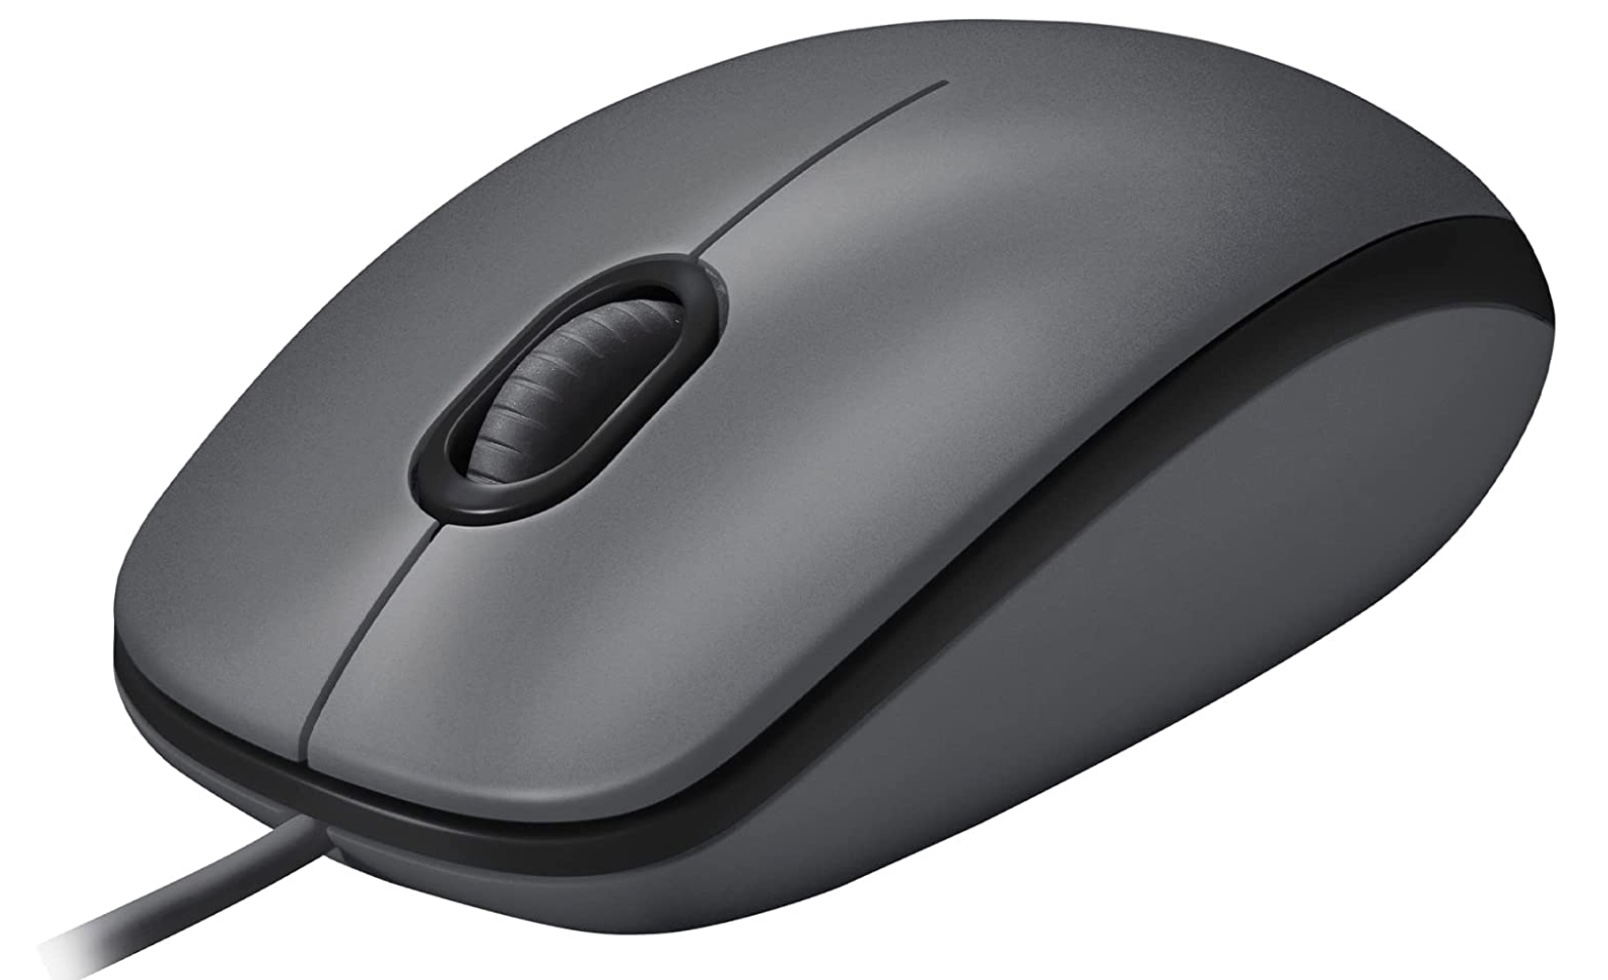
\includegraphics[width=0.2\textwidth]{Images/Mouse}} \\
	1      & Wired USB Mouse   
	& \href{https://www.amazon.de/-/en/Logitech-Buttons-Optical-Tracking-Compatible/dp/B07W8LZB2L/ref=sr_1_3?crid=WBB6LKE33KPR&keywords=kabelgebundene+usb+maus&qid=1675603667&sprefix=wired+usb+mouse%2Caps%2C135&sr=8-3}{Amazon.de} 
	&  12{,}85 \texteuro \\ \hline \\
	\multicolumn{4}{c}{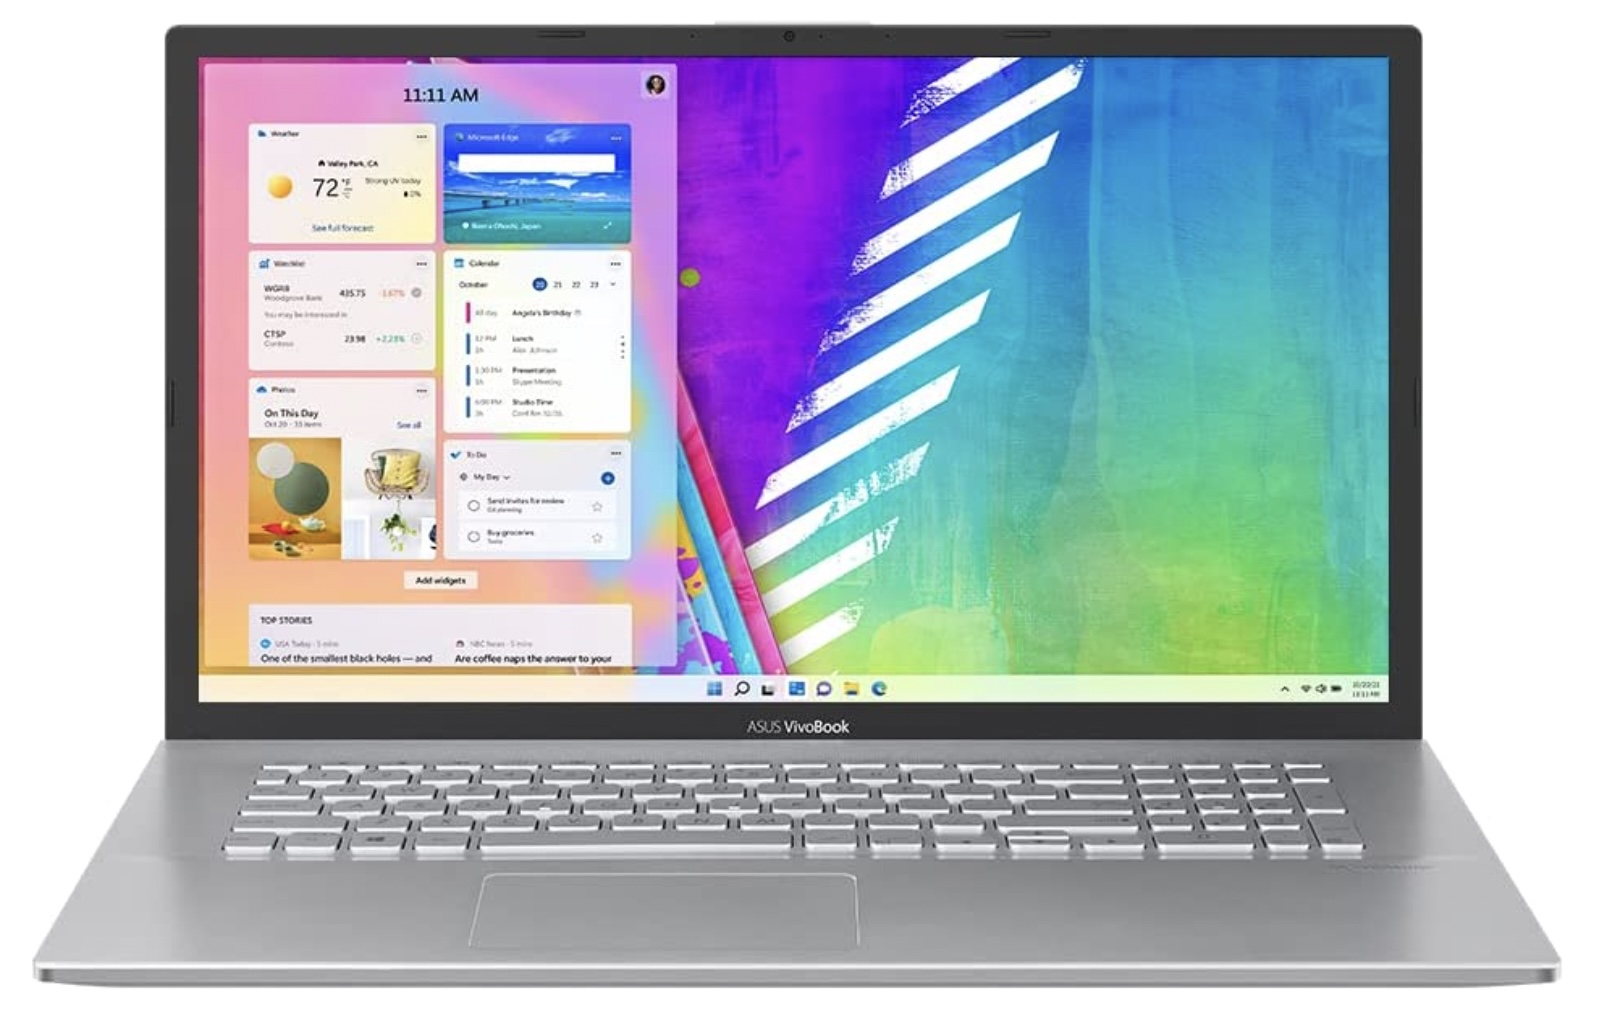
\includegraphics[width=0.2\textwidth]{Images/Laptop}} \\
	1      & Computer Laptop 
	& \href{https://www.amazon.de/-/en/Vivobook-Display-i7-1065G7-Keyboard-Transparent/dp/B0B9XXTN28?ref_=Oct_d_obs_d_427957031_4&pd_rd_w=S4jjh&content-id=amzn1.sym.e1b6b65c-25f7-4c64-bdd9-678097739641&pf_rd_p=e1b6b65c-25f7-4c64-bdd9-678097739641&pf_rd_r=682CQ3C074SF206E187V&pd_rd_wg=O3EMh&pd_rd_r=d9336b36-774e-44c4-a838-9c28fa27e899&pd_rd_i=B0B9XXTN28}{Amazon.de} 
	&  649 \texteuro \\ \hline \\	
	
	\multicolumn{4}{c}{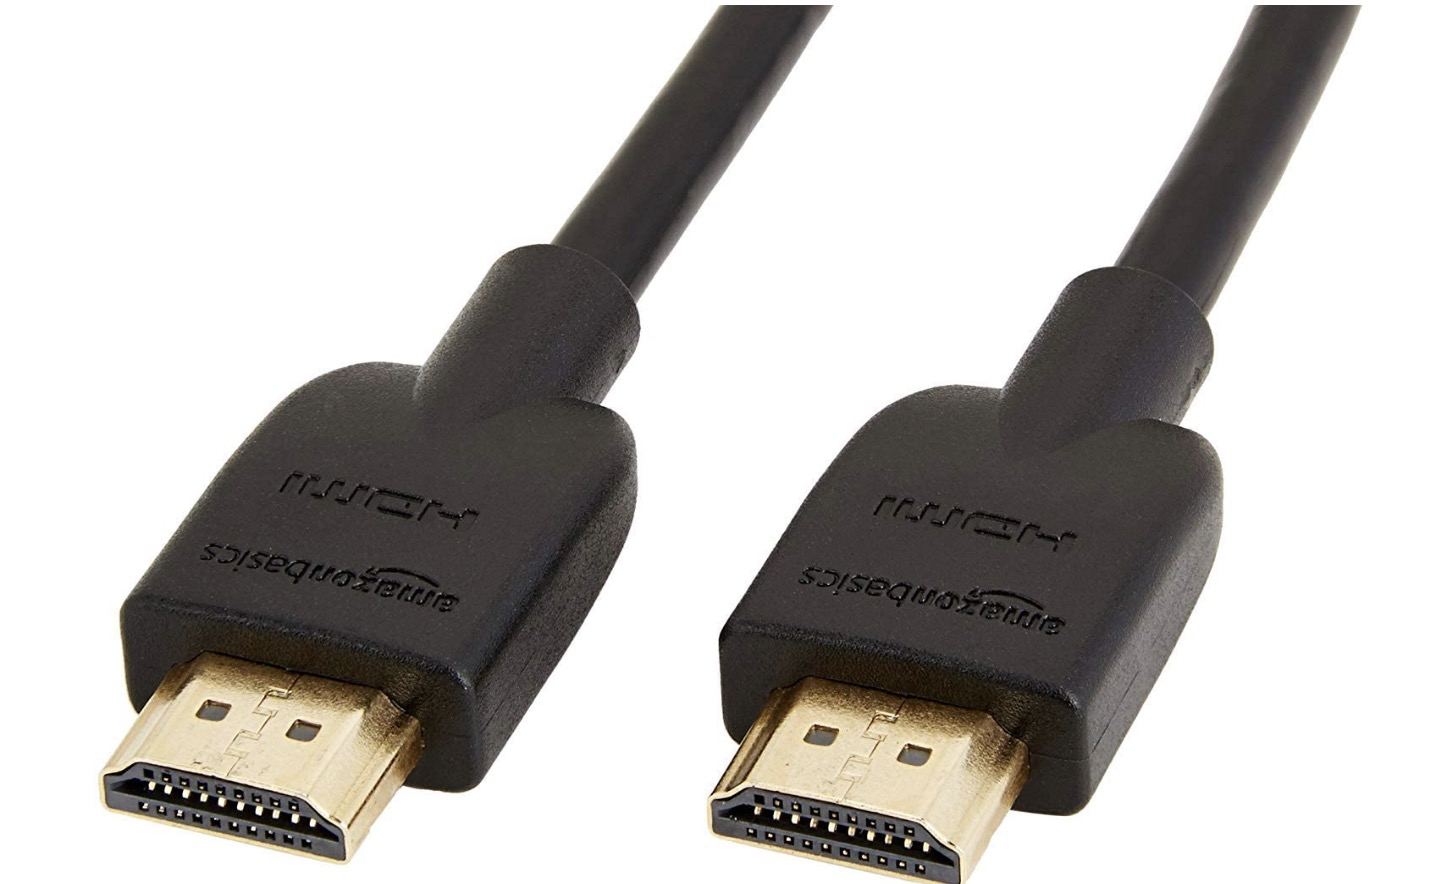
\includegraphics[width=0.2\textwidth]{./Images/HDMI}} \\
	1      & HDMI Cable
	& \href{https://www.amazon.de/Amazon-Basics-Supports-Format-Channel-black/dp/B014I8SIJY/ref=sr_1_1_ffob_sspa?crid=I3OG0691SCY3&keywords=hdmi-kabel&qid=1683184544&sprefix=hdmi%2Bcable%2Caps%2C96&sr=8-1-spons&sp_csd=d2lkZ2V0TmFtZT1zcF9hdGY&th=1}{Amazon.de}
	&  7{,}69 \texteuro \\ \hline
\end{longtable}


\section{Software Requirement and Bill Of Material }

%In this project for working with \ac{incs2} and Raspberry PI 3, we shall need softwares for these respective hardwares, along with installation of Python libararies for the purposes of model training. The model once trained, needs to be deployed into the INCS2 stick. For deployement into hardware, we shall need some softwares specifically designed for the purpose. In the following two tables, we shall look at libraries {table: \ref{table:PDF}} and softwares {table:\ref{table:SW version}} which will be used in the Project.


\begin{table}[ht]
	\caption[Libraries required with their respective versions]{Libraries required with their respective versions.} % title of Table
	\centering % used for centering table
\begin{tabular}{|l|l|}
	\hline
	\textbf{Library Version} & \textbf{Version} \\ \hline
	Python & 3.9.13 \\ \hline
	Pandas (Default library) & 1.4.4 \\ \hline
	Scikitlearn (Default library) & 1.0.2 \\ \hline
	Numpy (Default library) & 1.23.5 \\ \hline
	Matplotlib (Default library) & 3.5.2 \\ \hline
	Scipy (Default library) & 1.9.1 \\ \hline
	Statsmodels (Default library) & 0.13.2 \\ \hline
	Plotly & 1.1.0 \\ \hline
	Datetime (Default library) & 3.9.13 \\ \hline
	Lightgbm & 1.2.0 \\ \hline
\end{tabular}
	\label{table:PDF} % is used to refer this table in the text
\end{table}

\subsection{Python and Python Libraries Description }

AI and ML projects need certain technologies, these can be provided by Python. As Python is a stable programming language, it is flexible and has available tools The wide range of libraries is one of the main reasons why Python is the most popular programming language for AI and ML. Python langugage syntax is easier compared to other langauges, which aids people to quickly learn python and then use it for learning ML and AI. Morevover, solutions developed with Python can be built and also can run on multiple operating system platforms like Linux, MacOS, Windows etc. Therefore, in this project, Python was used as a programming language.\\

Python packages makes it easier to manage important processes such as analyzing and visualizing data, creating machine learning models, capture unstructured data from the web, and efficiently processes image and text information. In the Project, although many packages are used, we shall describe a few python libraries which are critical for important aspects of the Project.

\subsection{Applications}

	\begin{enumerate}
		
		\item \textbf{GitHub}
			
			GitHub is a widely used web-based platform for version control and collaboration, primarily focused on software development. It offers several features and benefits that make it an invaluable tool for managing software projects. 
			
			\begin{itemize}
				
				\item GitHub provides robust version control capabilities, allowing developers to track changes, collaborate effectively, and maintain a history of project modifications.
				
				\item GitHub facilitates seamless collaboration among team members.
				
				\item It offers built-in issue tracking functionality, allowing teams to create, assign, and track issues or bugs.
				
				\item GitHub's pull request mechanism facilitates code reviews, enabling developers to review proposed changes, provide feedback, and suggest improvements. 
				
				\item GitHub hosts millions of open source projects, making it a vibrant community for developers. It encourages collaboration, code sharing, and contribution to open source projects.
				
			\end{itemize}
			
		\item \textbf{Pycharm}
		
			PyCharm is an integrated development environment (IDE) specifically designed for Python programming. Developed by JetBrains, PyCharm offers a comprehensive set of tools and features that enhance productivity, simplify development workflows, and support efficient software development practices. It is widely recognized and preferred by Python developers for its powerful capabilities and user-friendly interface.
			
			\begin{itemize}
				
				\item PyCharm offers a robust code editor with syntax highlighting, code completion, and error detection, enabling developers to write Python code efficiently. 
				
				\item It includes a feature-rich debugger that allows developers to step through their code, set breakpoints, inspect variables, and analyze program flow.
				
				\item PyCharm seamlessly integrates with popular Python testing frameworks, such as unittest, pytest, and doctest.
				
				\item It offers integration with various version control systems, including Git, Mercurial, and Subversion.
				
			\end{itemize}
		
		\item \textbf{Anaconda}
		
			Anaconda is an open-source distribution of the Python and R programming languages for scientific computing, data science, and machine learning. It is a comprehensive platform that includes a package manager, environment manager, and a collection of over 1,500 pre-compiled libraries and tools. Anaconda provides a convenient way to install and manage Python/R packages, dependencies, and environments for data analysis and scientific computing projects. It also comes with the Anaconda Navigator, a graphical user interface (GUI) that allows users to easily access and manage their installed packages, environments, and development tools. Anaconda is widely used in the data science community due to its ease of use, cross-platform compatibility, and extensive library support.
			
	\end{enumerate}

\section{Requirements}

	The SalesPrediction project is developed using Python 3.10.11 within the Anaconda environment located at 
	\begin{verbatim}
		D:\Users\deeptihegde\anaconda3\envs\SalesPrediction
	\end{verbatim}
	The SalesPrediction project aims to predict sales using various machine learning techniques. The project has the following dependencies:
	
	\begin{itemize}
		
		\item bzip2 (version 1.0.8): Used for compression and decompression of files.
		
		\item ca-certificates (version 2023.05.30): Provides a set of trusted certificate authorities.
		
		\item libffi (version 3.4.4): Implements the Foreign Function Interface for various programming languages.
		
		\item openssl (version 3.0.9): Provides cryptographic functionalities and SSL/TLS protocols.
		
		\item pip (version 23.1.2): The package installer for Python.
		
		\item python (version 3.10.11): The Python programming language (version 3.10).
		
		\item setuptools (version 67.8.0): Used for packaging Python distributions.
		
		\item sqlite (version 3.41.2): A self-contained, serverless, and zero-configuration SQL database engine.
		
		\item tk (version 8.6.12): Provides the Tk GUI toolkit for Python applications.
		
		\item vc (version 14.2): The Visual C++ Build Tools.
		
		\item vs2015\_runtime (version 14.27.29016): The Visual Studio 2015 C++ runtime library.
		
		\item wheel (version 0.38.4): A built-package format used for Python distributions.
		
		\item xz (version 5.4.2): A compression library and command-line tool.
		
		\item zlib (version 1.2.13): A data compression library.
		
		\item The project also utilizes several Python packages installed via pip:
		
		\begin{itemize}
			
			\item contourpy (version 1.1.0): A package for creating contour plots.
			
			\item cycler (version 0.11.0): Provides composable cycle classes.
			
			\item fonttools (version 4.40.0): A library for manipulating fonts.
			
			\item joblib (version 1.2.0): Provides tools for parallel computing and caching.
			
			\item kiwisolver (version 1.4.4): Solves linear programming problems.
			
			\item matplotlib (version 3.7.1): A plotting library for Python.
			
			\item numpy (version 1.25.0): A powerful numerical computing library.
			
			\item packaging (version 23.1): Provides utilities for Python package metadata.
			
			\item pandas (version 2.0.2): A versatile data analysis and manipulation library.
			
			\item pillow (version 9.5.0): Adds image processing capabilities to Python.
			
			\item pyparsing (version 3.1.0): A general-purpose parsing library.
			
			\item python-dateutil (version 2.8.2): Provides date and time utilities for Python.
			
			\item pytz (version 2023.3): A library for timezone calculations.
			
			\item scikit-learn (version 1.2.2): A machine learning library for Python.
			
			\item scipy (version 1.11.0): A scientific computing library.
			
			\item six (version 1.16.0): A Python 2 and 3 compatibility library.
			
			\item sklearn (version 0.0.post5): Provides a consistent API for various machine learning algorithms.
			
			\item threadpoolctl (version 3.1.0): A library for dynamic threadpool management.
			
			\item tzdata (version 2023.3): Timezone database for Python.
			
			\item xgboost (version 1.7.6): A gradient boosting library.
			
		\end{itemize}
		
	\end{itemize}
